% Preamble
\documentclass[11pt]{article}
\usepackage{braket}
\usepackage{graphicx}
\usepackage[margin=1in]{geometry}

\usepackage{makeidx}  % allows for indexgeneration
\usepackage{ifpdf}
\usepackage{url}


\title{Elementary Cellular Automata as an Error Minimized Hash}
\date{November 2024}
\author{Daniel McKinley}

% Document
\begin{document}

\maketitle

\section{Introduction}

Elementary cellular automata (ECA) are 8 bit extensions of 4 bit logic gate truth tables, done linearly in parallel. \cite{Wolfram}
Here a subset of 8 of the 256 ECA rules are explored as a cryptographic hash function that tracks the Fast Fourier Transform (FFT) and Fast Walsh-Hadamard Transform. General algorithm, specific ECA rules, and aggregate properties are discussed. It is implemented in Java at \cite{mygit} along with a sample of the algorithm operating on a given bitmap image at the website in the references. \\
\section{Main Algorithm}


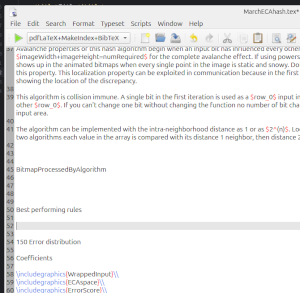
\includegraphics{testScreenshot}\\
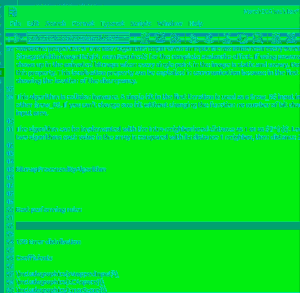
\includegraphics{processedDepth1}\\
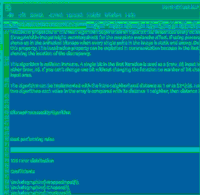
\includegraphics{processedDepth3}\\
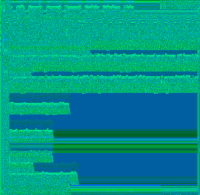
\includegraphics{processedDepth6}\\
Include graphics for: Input example, Codeword output example, Error map example\\
BitmapProcessedByAlgorithm\\

\begin{center}
there are $2^(16)=65536$ binary 4x4 arrays\\
 where there are $2^(4)$ possible $row_0$ neighborhoods for a given ECA rule\\
 each of these 16 input-ECAoutput arrays are scored by\\
\[  \sum_{r=0}^{3} \sum_{c=0}^{3} 2^r ( compressionAttempt_{r c} \oplus original_{r c}) \]\\
 the value of the neighborhoods of the minimum and maximum of these 16 sums \\
 are noted as the solution for the original binary matrix  \\
\end{center}
The algorithm works on $2^n*2^n$ square matrices,2x2, 4x4, 8x8. For all $2^(16)=655536$ possibilities of a 4x4 binary array, create a wrapped 4x4 array, use row 0 as all possible $2^4=16$ input neighborhoods, calculate the remaining three rows for all 16 possible input values using a Wolfram code. For each of all these 16 possible inputs, score the 4x4 array with a weighted sum of discrepancies between this codeword-produced output and the original 4x4 matrix Input[][]. The lowest and highest scoring neighborhood are then two length-four codewords for a possible neighborhood of size 4x4. The algorithm's solutions for all neighborhoods of a certain size become a hexadecimal Wolfram code for a small QR code. Changing the size is not fully studied due to computing constraints of mapping all $2^(64)$ possible 8x8 matrices on up. The paper assumes a square input matrix, the algorithm is implemented for any number of rows and columns. \\
\begin{center}
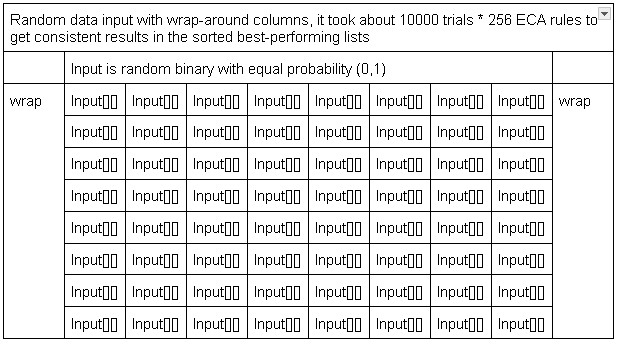
\includegraphics{WrappedInput}\\
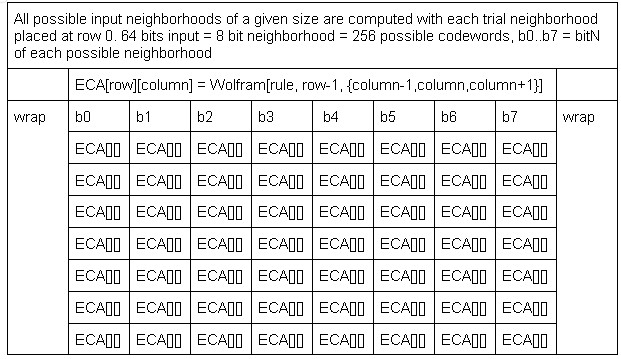
\includegraphics{ECAspace}\\
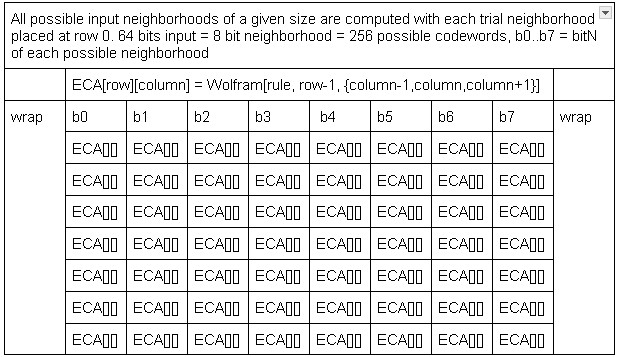
\includegraphics{ErrorScore}\\
\end{center}

Doing this algorithm for every cell in a bitmap quadruples its size. After an initilization frame, the algorithm is applied to every cell in the bitmap with the neighborhood square's rows and columns operating on a $2^depth$ basis. Frame one's neighborhoods are next door neighbors, frame two's neighbors are two doors away, frame four's are four, then eight and so on. This comparison of neighbors of distance $2^n$ is similar to the FFT and Fast Walsh-Hadamard process.\\

This algorithm can both minimize the errorScore in a lossy compression, and maximizing the errorScore.\\

There are 8 [0,15,51,85,170,204,240,255] of the 256 8 bit ECA truth tables that display the properties of unique codewords for any given input and perfectly even distribution of codewords. 0 and 255 are included because in the 4 rows of the output matrix, 1 is neighborhood input and 3 are output, and still produce an errorScore. This subset works with both errorScore minimization and errorScore maximization. These two min max 8-tuples are implemented as a cryptographic hash.\\

Avalanche properties of this hash algorithm begin when an input bit has influenced every other input bit. If using sequential hashes, you need $imageWidth+imageHeight=numRequired$ for the complete avalanche effect. If using powers of two the avalanche effect begins at $log_2 (width) + log_2 (height)$. This property shows up in the animated bitmaps when every single point in the image is static and snowy. Doing fewer iterations than the avalanche's diffusion threshold but more than zero limits this property. This localization property can be exploited in communication because in the first few iterations the data is irreversible enough to be imperfectly unencryptable while showing the location of the discrepancy.\\

This algorithm has minimum collision resistance. The initial conversion from 4 hexadecimal places to 1 hexadecimal place mean every output 0-15 has 4096 other neighborhoods that produce the same thing. A general method of producing these collisions on command is under investigation.\\

The algorithm can be implemented with the intra-neighborhood distance as 1 or as $2^(n)$. Loops in the implementation using the powers 2 directly parallel the FFT and FWH. In those two algorithms each value in the array is compared with its distance 1 neighbor, then distance 2, then distance 4, then 8, then 16 and so on.\\

The weight in the errorScore sum can be $2^(row($ or $2^(column)$, both produce the same set of 8 tuples with the unique solution property, though other ECA rule's properties don't necessarily carry over.\\

The size of the input array can be easily be any power of 2 squared. Wolfram code lengths of $2^(16)$ are acceptable, lengths of $2^(64)$ are in principle doable but not practical. The 8 tuple's uniqueness and distribution properties may apply at size 8 squared, it may not; it is only completely tested for size 4. Running statistics on random samples of size 8 have not been done yet.\\

Best performing rules\\

150 Error distribution\\

Reconstruction\\

voting() subfunction to increase accuracy\\



\bibliographystyle{plain}
\bibliography{HashBib.bib}

\end{document}